\documentclass[conference]{IEEEtran}
\IEEEoverridecommandlockouts

\usepackage{cite}
\usepackage{amsmath,amssymb,amsfonts}
\usepackage{graphicx}
\usepackage{booktabs}
\usepackage{multirow}
\usepackage{float}
\usepackage{url}
\usepackage[hidelinks]{hyperref}

\graphicspath{{../results/figures/}}

\begin{document}

\title{Coverage-Guided Search-Based Test Generation for a Tennis Scoring
Engine: A Two-Regime Comparison Against Random Testing}

\author{\IEEEauthorblockN{Alessandro Ligugnana, Gianluca Fava}
\IEEEauthorblockA{Software Testing --- Track B}}

\maketitle

\begin{abstract}
Search-based test generation guided by code coverage is a well established
technique, yet its advantage over plain random testing is known to depend on
the difficulty of the search problem. We study a coverage-guided evolutionary
test generator for a tennis scoring engine, a compact state-machine subject
under test (SUT) with branching logic for deuce, tie-breaks and three
tournament rulesets. We compare it against a random baseline and an ablation
that keeps the evolutionary machinery but removes the coverage-guided fitness,
under a two-regime budget design with $N{=}30$ repetitions, measuring branch
coverage and mutation score with Mann--Whitney $U$ tests and
Vargha--Delaney $A_{12}$ effect sizes. Random testing is competitive with, and
frequently superior to, the guided search at every budget. The value of the
coverage-guided fitness emerges instead against the unguided evolutionary
baseline, where it grows with the budget and reaches a \emph{large} effect on
mutation score. We discuss why coverage saturation on small subjects
neutralises guidance relative to random testing, and what this implies for when
search-based testing is worth its cost.
\end{abstract}

\begin{IEEEkeywords}
search-based software testing, branch coverage, mutation testing, random
testing, ablation study, empirical evaluation.
\end{IEEEkeywords}

\section{Introduction}
Automated test generation aims to produce test suites that exercise a program
thoroughly with little human effort. Search-based software testing (SBST) casts
this as an optimisation problem in which candidate test inputs are evolved to
maximise a coverage-oriented fitness function~\cite{mcminn2004search,
fraser2011evosuite}. A recurring and practically important question is whether
the guidance provided by such a fitness function actually outperforms undirected
\emph{random} testing, which is known to be surprisingly competitive on simple
domains~\cite{arcuri2012random}.

We investigate this question on a tennis scoring engine: a deterministic state
machine whose control flow encodes the non-trivial rules of tennis (game,
deuce/advantage, set, tie-break) and three tournament rulesets that differ in
the decisive-set tie-break. The SUT is small but branch-rich, which makes it a
clean testbed for isolating the contribution of coverage guidance. We compare
three generators at equal budget: a coverage-guided evolutionary algorithm, a
random baseline, and an \emph{ablation} that retains the evolutionary structure
but replaces the fitness with a constant, thereby isolating the effect of the
fitness function itself.

We frame the study with the Goal--Question--Metric paradigm. The \emph{goal} is
to assess whether, and under which conditions, coverage-guided search improves
test effectiveness over random testing for the tennis engine. We measure
effectiveness through branch coverage (a structural proxy) and mutation score
(a fault-detection proxy~\cite{just2014mutants}). The research questions are:

\begin{itemize}
\item \textbf{RQ1.} Does coverage-guided generation achieve higher branch
coverage and mutation score than random testing at equal budget?
\item \textbf{RQ2 (ablation).} Is any observed contribution attributable to the
coverage-guided fitness, or merely to the evolutionary structure?
\item \textbf{RQ3 (regime).} How does the advantage of guidance vary with the
search budget?
\end{itemize}

The main finding is a two-regime picture. Random testing is competitive or
superior on both metrics across all budgets, because coverage saturates quickly
on this small SUT. The fitness function nonetheless has a real and growing
effect \emph{relative to the unguided baseline}, becoming a \emph{large} effect
on mutation score at medium-to-high budgets. We report all numbers honestly,
including the negative result for RQ1.

\section{Related Work}
Search-based test generation has been studied extensively since the survey of
McMinn~\cite{mcminn2004search}. Tools such as EvoSuite~\cite{fraser2011evosuite}
generate whole test suites for object-oriented programs by optimising a coverage
criterion, and many-objective formulations such as
MOSA~\cite{panichella2018mosa} treat individual coverage targets as separate
objectives to steer the search toward hard-to-reach branches. The
competitiveness of random testing against more sophisticated strategies is a
recurring theme: Arcuri et al.~\cite{arcuri2012random} give theoretical and
empirical conditions under which random testing is effective, showing that on
many problems the probability of covering targets by chance is high enough to
make guidance unnecessary. Our study is methodologically aligned with the
guidelines of Arcuri and Fraser~\cite{arcuri2014hitchhiker} for assessing
randomised algorithms, using repeated runs, non-parametric tests and
standardised effect sizes~\cite{vargha2000critique}. We adopt mutation analysis
as a fault-detection proxy following the evidence of
Just et al.~\cite{just2014mutants} that mutant detection correlates with real
fault detection. Our contribution is not a new algorithm but a controlled,
ablated comparison on a compact, fully specified SUT, together with a two-regime
budget analysis that isolates when coverage guidance pays off.

\section{Subject Under Test}
The SUT is a single-module tennis scoring engine
(\texttt{src/tennis\_engine.py}). The public API follows an internal contract:

\begin{itemize}
\item \texttt{TennisMatch(ruleset)} with
\texttt{ruleset}~$\in$~\{\texttt{wimbledon}, \texttt{usopen},
\texttt{ausopen}\};
\item \texttt{play\_point(winner)} drives the engine with
\texttt{winner}~$\in$~\{\texttt{"A"},\texttt{"B"}\}, raising
\texttt{ValueError} for an invalid winner and \texttt{RuntimeError} if called
after the match ends;
\item \texttt{score()} returns a dictionary with exactly the keys
\texttt{points}, \texttt{games}, \texttt{sets}, \texttt{in\_tiebreak},
\texttt{is\_over}, \texttt{winner}.
\end{itemize}

The engine implements best-of-three matches. A game is won at four points with a
two-point margin (deuce/advantage); a set is won at six games with a two-game
margin, at $7$--$5$, or through a tie-break at $6$--$6$. The three rulesets
differ \emph{only} in the decisive-set tie-break target: Wimbledon and
Australian Open use a $10$-point tie-break (two-point margin), the US Open a
standard $7$-point tie-break. Scoring logic is written with explicit
\texttt{if/elif} chains, intentionally producing a diverse set of branches for
deuce, advantage, the $7$--$5$ and $7$--$6$ set endings, and the per-ruleset
tie-break targets. Under \texttt{coverage.py} in branch mode the module exposes
66 branch arcs in total. A test input is simply a sequence of point winners,
i.e.\ a list over \{\texttt{A},\texttt{B}\}; the search space is the set of such
sequences up to a maximum length.

\section{Approach}

\subsection{Random baseline}
The random generator emits \texttt{budget} independent sequences of point
winners; each sequence has a uniformly random length in $[4, 400]$ and each
point is drawn uniformly from \{\texttt{A},\texttt{B}\}. It is fully
deterministic given the seed (a local \texttt{random.Random(seed)} instance is
used throughout), which guarantees reproducibility.

\subsection{Coverage-guided search}
The search generator is an evolutionary algorithm over sequences of point
winners. It initialises a population of random sequences, then repeatedly:
(a)~executes each candidate and (b)~scores it; (c)~selects elites by fitness;
(d)~produces offspring by mutation and crossover. The mutation operators are
point \emph{flip}, \emph{insert}, \emph{delete}, contiguous \emph{block-replace}
and suffix \emph{extend}; single-point crossover recombines two elites. Every
evaluated sequence is accumulated in an \emph{archive}, which constitutes the
returned test suite. The configuration is summarised in
Table~\ref{tab:params}.

\begin{table}[t]
\centering
\caption{Evolutionary algorithm configuration.}
\label{tab:params}
\begin{tabular}{ll}
\toprule
Parameter & Value \\
\midrule
Population size & 8 \\
Elite ratio & 0.3 \\
Crossover probability & 0.3 \\
Sequence length range & $[4, 400]$ \\
Budget (fitness evaluations) & $\{20, 60, 200\}$ \\
Repetitions per cell & $N=30$ \\
\bottomrule
\end{tabular}
\end{table}

The fitness of a candidate combines its own branch coverage with a novelty
bonus for arcs not yet in the archive:
\[
\mathit{fitness}(s) = |C(s)| + |C(s)\setminus A|,
\]
where $C(s)$ is the set of branch arcs covered by $s$ and $A$ is the running
archive of covered arcs. The own-coverage term is deliberate: a fitness based on
novelty \emph{alone} collapses to zero for every candidate as soon as the
archive saturates, which on a small SUT happens within the first generation and
removes all selection pressure. The combined form keeps a non-zero gradient
throughout the search and is what makes the guided search differ from the
ablation in practice.

\subsection{Ablation}
The ablation generator is the \emph{same} algorithm as the search generator,
invoked with a constant fitness ($\equiv 0$). It is implemented by delegating to
the search generator and injecting the constant fitness function, so that
population, selection, mutation and crossover operators, number of generations,
and random-number usage are identical; only the fitness differs. This guarantees
that any difference between search and ablation is attributable to the
coverage-guided fitness and to nothing else. With a constant fitness the
selection has no signal and the search degenerates into an unguided walk over the
operator space. We verified empirically that the two generators produce distinct
suites at budgets that allow at least one generation of offspring, and that all
three generators are deterministic given the seed.

\subsection{Oracle of the generated tests}
Mutation score is only meaningful with a strong oracle. We therefore translate
each generated sequence into a test that, \emph{after every} \texttt{play\_point}
call, asserts state \emph{invariants} of the contract rather than hard-coded
expected scores (which are unknown a priori for generated sequences). The
invariants include: the exact key set of \texttt{score()}; integer ranges for
sets ($0\!\le\!\cdot\!\le\!2$, sum $\le 3$) and games ($0\!\le\!\cdot\!\le\!7$);
admissible point tokens (\{\texttt{0},\texttt{15},\texttt{30},\texttt{40},
\texttt{Ad}\} in a game, non-negative integers in a tie-break); consistency
between \texttt{is\_over} and \texttt{winner}; monotonicity of the aggregate set
and (within a set) game counts; terminal behaviour (a further point after the
match is over must raise \texttt{RuntimeError}); and rejection of invalid input.
A \emph{null} oracle (e.g.\ asserting only that \texttt{score()} is not
\texttt{None}) can kill only mutants that crash the execution; it cannot detect
mutants that silently corrupt the score, which is precisely what the invariant
oracle catches. The choice of oracle is therefore a first-order factor for the
mutation score and is held identical across all three generators.

\subsection{Coverage measurement}
Branch coverage is measured with \texttt{coverage.py} in branch mode, targeting
only the engine module, through the JSON report API. Each measurement uses a
\emph{fresh} \texttt{Coverage} instance and reports from in-memory data, so there
is no coverage leakage across runs. The total number of branch arcs (66) is
constant across all runs, as expected for a fixed SUT.

\section{Experimental Setup}
We run a full factorial design over three generators (\texttt{random},
\texttt{search}, \texttt{ablation}), three rulesets, and three budgets, with
$N{=}30$ independent seeds per cell, for $810$ runs in total. The two-regime
design contrasts a low budget, where random testing does \emph{not} saturate
coverage, against a high budget; we additionally include an intermediate budget
to trace the transition. The budgets are $\{20, 60, 200\}$ candidate
evaluations.

Budget is operationalised as the number of candidate sequences a generator may
consider, and all generators return a suite of $\approx\!\mathit{budget}$
sequences, so the final measured suites have the same size. Tooling:
\texttt{coverage.py} (branch mode), \texttt{mutmut}~v3 for mutation analysis,
\texttt{scipy} for the statistics; Python~3.10. For each run we record branch
coverage, mutation score, and wall-clock time.

\paragraph{Statistical analysis}
For each (budget, ruleset, metric) we compare \texttt{search} against
\texttt{random} and against \texttt{ablation} using the two-sided
Mann--Whitney $U$ test ($\alpha=0.05$) and the Vargha--Delaney $A_{12}$ effect
size~\cite{vargha2000critique,arcuri2014hitchhiker}. We classify $A_{12}$ with the
effect-size thresholds adopted in the course: for $A_{12}>0.5$,
$[0.50,0.56)$ is negligible, $[0.56,0.64)$ small, $[0.64,0.71)$ medium and
$>0.71$ large; the bands are symmetric below $0.5$ (equivalently, negligible
for $|A_{12}-0.5|<0.06$, small for $<0.14$, medium for $<0.21$, large
otherwise). $A_{12}>0.5$ favours \texttt{search}; $A_{12}<0.5$ favours the
comparison baseline.

\paragraph{Threats to validity}
\emph{Construct.} Branch coverage is a structural proxy and mutation score a
fault proxy; both are imperfect, though mutation score is an established
predictor of real fault detection~\cite{just2014mutants}. Branch coverage is
moreover operationalised by driving the SUT through \texttt{play\_point} only:
the branches of \texttt{score()} (point/score formatting) and the error paths
are not exercised by this measurement harness, so the reported figures
\emph{under}-estimate the coverage actually achieved by the generated suites,
which call \texttt{score()} after every point and reach $\approx0.97$; since all
generators are measured identically, this does not affect their relative
ranking. Finally, two arcs---the $7$--$5$ set-win case in
\texttt{\_check\_set\_over}---are dead code, dominated by the general
``$\ge\!6$ games with a two-game margin'' rule and hence logically unreachable,
so they cap the attainable coverage below $1.0$ for every generator.
\emph{Internal.} Budget is operationalised as the number of candidate sequences,
so the measured suites have equal size; the coverage-guided search, however,
executes the SUT once per fitness evaluation
($\approx\!\mathit{budget}$ additional SUT executions) to obtain the coverage
signal, a cost not paid by the random baseline. This asymmetry, if anything,
favours the baseline, because at equal budget the guided search returns
\emph{fewer} unique sequences (mutation and elitism create duplicates); the
comparison is therefore fair to conservative with respect to \texttt{search}.
\emph{External.} A single, small SUT limits generalisability; results may differ
on larger programs with harder-to-cover branches.
\emph{Conclusion.} We mitigate randomness with $N{=}30$ repetitions and
non-parametric tests with effect sizes.

\section{Results}
Coverage and mutation-score medians are essentially invariant across the three
rulesets (the rulesets differ only in a rarely-reached decisive tie-break); we
therefore report representative medians in Table~\ref{tab:medians} and the
statistical comparisons in Table~\ref{tab:stats}, noting that all three rulesets
agree on significance and effect-size class. Figures~\ref{fig:curve-mut}
and~\ref{fig:curve-cov} show the budget curves, and Fig.~\ref{fig:box} the
distribution at the highest budget.

\begin{table}[t]
\centering
\caption{Median branch coverage and mutation score per generator and budget
(representative ruleset; rulesets agree to within rounding).}
\label{tab:medians}
\begin{tabular}{llccc}
\toprule
Metric & Budget & \texttt{random} & \texttt{search} & \texttt{ablation} \\
\midrule
\multirow{3}{*}{Branch cov.}
 & 20  & 0.727 & 0.682 & 0.682 \\
 & 60  & 0.773 & 0.727 & 0.727 \\
 & 200 & 0.773 & 0.773 & 0.773 \\
\midrule
\multirow{3}{*}{Mutation}
 & 20  & 0.398 & 0.377 & 0.380 \\
 & 60  & 0.435 & 0.427 & 0.399 \\
 & 200 & 0.451 & 0.448 & 0.424 \\
\bottomrule
\end{tabular}
\end{table}

\begin{table}[t]
\centering
\caption{Statistical comparison (\texttt{search} vs.\ baseline). $p$:
Mann--Whitney $U$ (two-sided); $A_{12}$: Vargha--Delaney effect size
($>0.5$ favours \texttt{search}). Representative ruleset.}
\label{tab:stats}
\setlength{\tabcolsep}{4pt}
\begin{tabular}{llccl}
\toprule
Comparison & Budget & $p$ & $A_{12}$ & Effect \\
\midrule
\multicolumn{5}{l}{\emph{Branch coverage}}\\
search vs random   & 20  & $0.0005$ & 0.250 & large (random) \\
search vs random   & 60  & $0.0002$ & 0.258 & large (random) \\
search vs random   & 200 & $0.042$  & 0.433 & small (random) \\
search vs ablation & 20  & $0.93$   & 0.507 & negligible \\
search vs ablation & 60  & $0.21$   & 0.588 & small (search) \\
search vs ablation & 200 & $0.015$  & 0.642 & medium (search) \\
\midrule
\multicolumn{5}{l}{\emph{Mutation score}}\\
search vs random   & 20  & $5.4\mathrm{e}{-}5$ & 0.197 & large (random) \\
search vs random   & 60  & $0.070$  & 0.364 & small (random) \\
search vs random   & 200 & $0.0004$ & 0.240 & large (random) \\
search vs ablation & 20  & $0.51$   & 0.451 & negligible \\
search vs ablation & 60  & $2.4\mathrm{e}{-}5$ & 0.818 & large (search) \\
search vs ablation & 200 & $<\!10^{-6}$ & 0.882 & large (search) \\
\bottomrule
\end{tabular}
\end{table}

\begin{figure}[t]
\centering
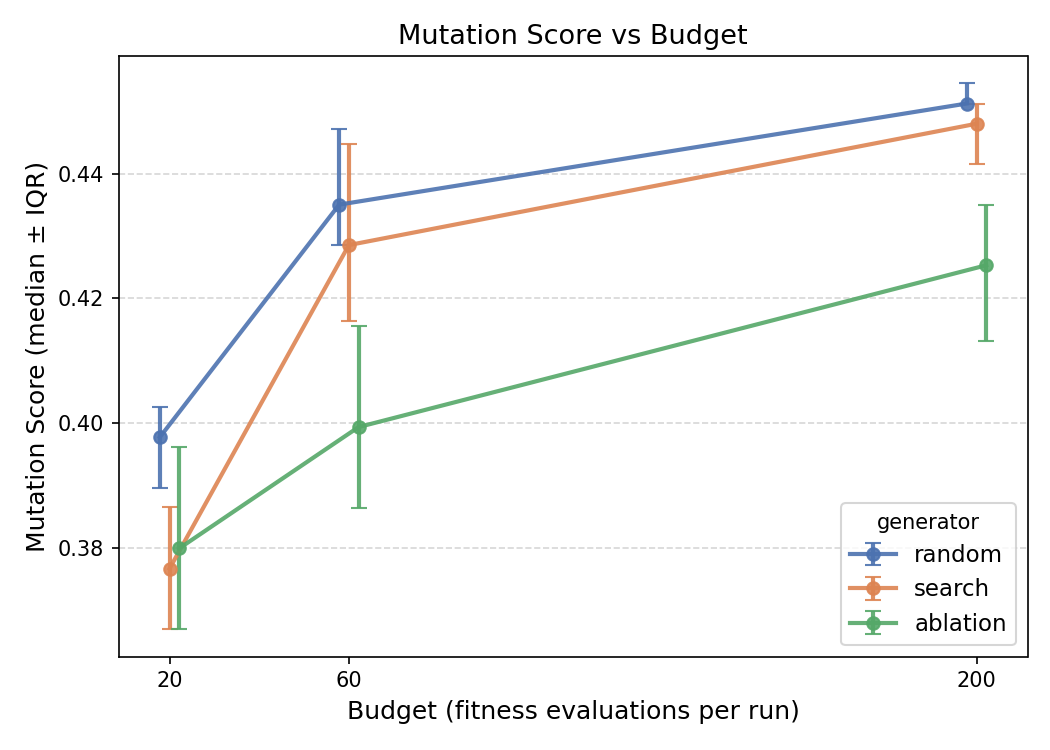
\includegraphics[width=\columnwidth]{budget_curve_mutation_score.png}
\caption{Mutation score (median $\pm$ IQR) versus budget. The guided search
tracks but does not exceed random; it separates clearly from the unguided
ablation as the budget grows.}
\label{fig:curve-mut}
\end{figure}

\begin{figure}[t]
\centering
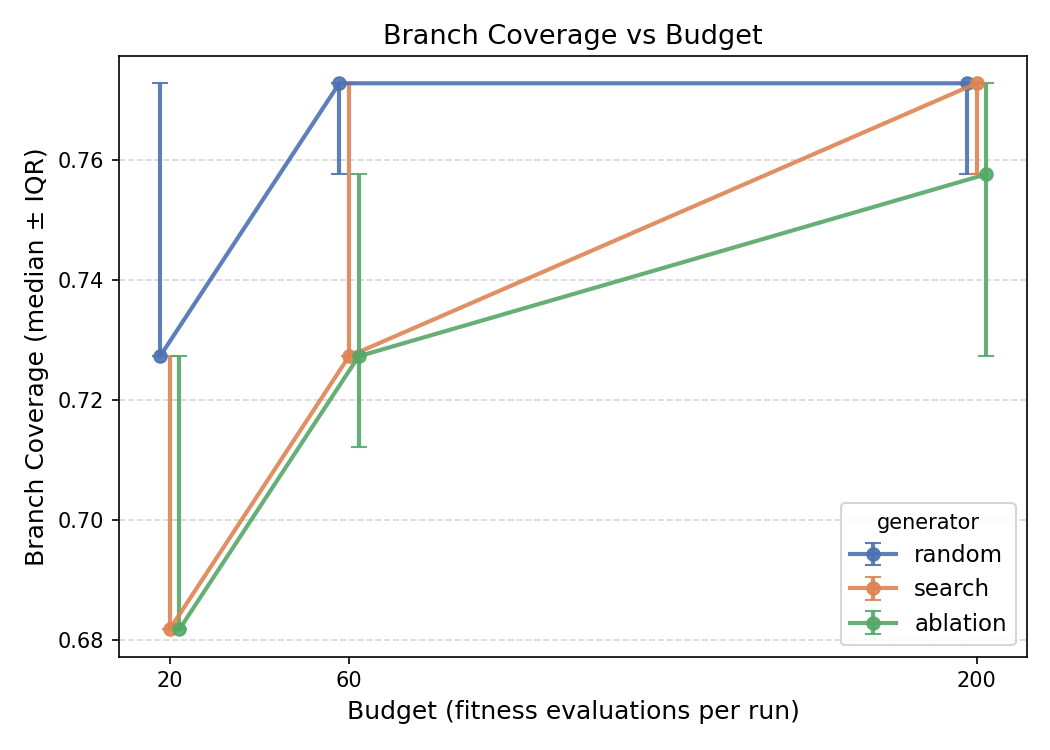
\includegraphics[width=\columnwidth]{budget_curve_branch_coverage.png}
\caption{Branch coverage (median $\pm$ IQR) versus budget. All generators
converge as coverage saturates at high budget; random leads at low and medium
budget.}
\label{fig:curve-cov}
\end{figure}

\begin{figure}[t]
\centering
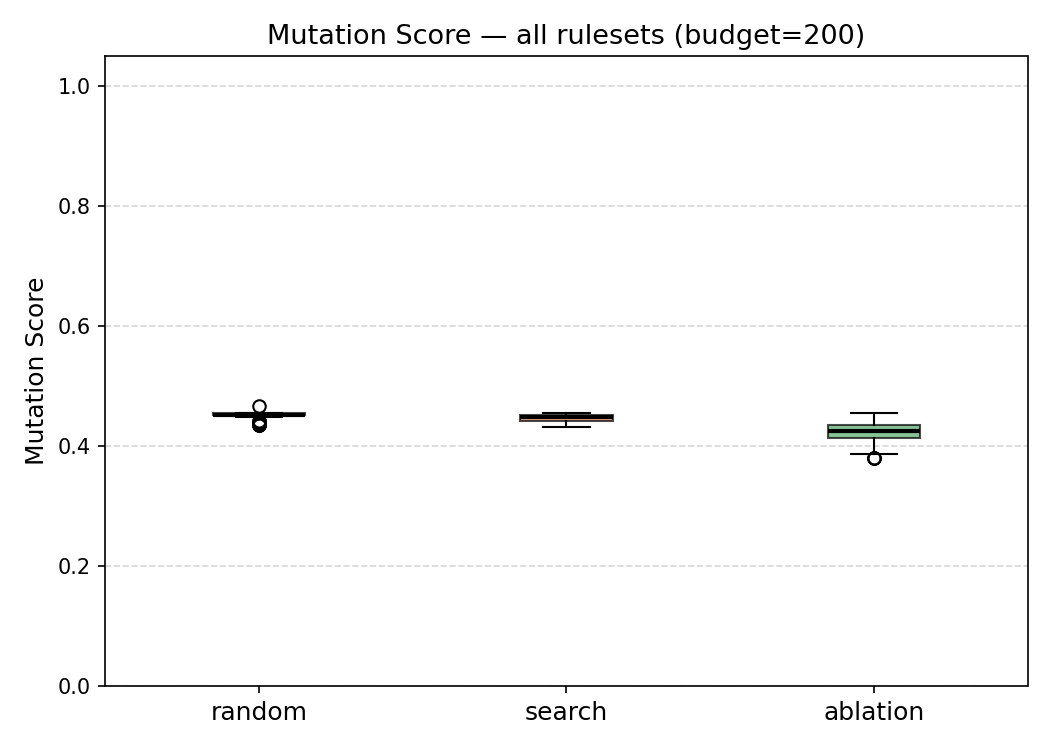
\includegraphics[width=\columnwidth]{boxplot_mutation_score_b200.png}
\caption{Mutation score distribution at budget 200 (all rulesets). The guided
search and random overlap, while the unguided ablation is clearly lower.}
\label{fig:box}
\end{figure}

\subsection{RQ1: search vs.\ random}
Coverage-guided search does \emph{not} outperform random testing. On branch
coverage, random is significantly better at budgets 20 and 60 (large effect,
$A_{12}=0.25$ and $0.26$) and the two converge at budget 200 ($A_{12}=0.43$,
small). On mutation score random is competitive or superior at every budget
($A_{12}=0.20$--$0.36$ favouring random); the gap is smallest and statistically
non-significant at budget~60 ($p=0.07$). The answer to RQ1 is therefore negative
for this SUT.

\subsection{RQ2: role of the fitness (ablation)}
The coverage-guided fitness has a clear effect once the search runs long enough
to breed offspring. On mutation score, \texttt{search} beats \texttt{ablation}
with a \emph{large} effect at budgets 60 and 200 ($A_{12}=0.82$ and $0.88$,
$p<10^{-4}$), and on branch coverage with a \emph{medium} effect at budget 200
($A_{12}=0.64$, $p=0.015$). At budget 20 the two are statistically
indistinguishable ($A_{12}\approx0.5$), because the budget is exhausted before
the first generation of guided offspring is produced. The fitness function thus
provides a genuine, increasing contribution---just not enough to overtake random.

\subsection{RQ3: effect of budget}
The advantage of guidance over the unguided baseline grows monotonically with
budget: negligible at 20, small-to-large at 60, large at 200
(Table~\ref{tab:stats}, Fig.~\ref{fig:curve-mut}). Against random, the picture is
the opposite of the naive expectation: increasing the budget lets random
saturate coverage and \emph{closes} any gap rather than opening one.

\subsection{Cost}
Guidance is not free. Averaged over runs, the search generator takes about
$+18\%$, $+22\%$ and $+28\%$ wall-clock time over random at budgets 20, 60 and
200 respectively (e.g.\ $72.9$\,s vs.\ $57.1$\,s at budget 200), reflecting the
extra SUT executions performed to compute the fitness.

\section{Discussion}
\paragraph{Why random saturates and neutralises guidance}
The SUT is small and its branches are reachable by moderately long random point
sequences: a single random sequence frequently plays a full match and exercises
deuce, set and tie-break logic. With independent sampling, a handful of such
sequences already cover most of the 66 arcs, so coverage saturates around $0.77$
regardless of guidance. This is the classic regime in which random testing is
hard to beat~\cite{arcuri2012random}: when the probability of covering a target
by chance is high, a fitness gradient adds little. The guided search, by
concentrating on a converging population, even explores \emph{fewer} distinct
states at equal budget, which explains why it does not exceed random.

\paragraph{Why coverage and mutation score can diverge}
Covering the branch that a mutant lives on is necessary but not sufficient to
kill it: the mutated state must also propagate to an assertion. The search's
tendency to converge reduces the diversity of game states reaching the oracle,
so even when branch coverage is matched, the guided suite may kill slightly fewer
mutants than a more diverse random suite. This decoupling between a structural
proxy and a fault proxy is well documented~\cite{just2014mutants} and is visible
here as the small but persistent random advantage on mutation score
(Fig.~\ref{fig:box}).

\paragraph{When guidance pays}
The ablation isolates what the fitness actually buys: a large mutation-score gain
over an unguided evolutionary search at sufficient budget. Guidance therefore
\emph{does} steer the search toward more effective tests; its failure to beat
random is a property of the \emph{subject} (cheap-to-cover), not of the fitness.
We would expect the ranking to invert on subjects where targets are rare relative
to the budget, i.e.\ where random rarely hits the hard branches and a gradient
becomes decisive~\cite{mcminn2004search,panichella2018mosa}.

\paragraph{Practical implication}
Search-based testing is worthwhile when the search space is large or hard
relative to the available budget; on cheap-to-cover subjects it adds a measurable
time overhead ($\sim\!28\%$ here) without improving effectiveness over random.
Practitioners should size the budget and choose between random and guided search
according to how easily targets are reached.

\section{Conclusion}
We presented a two-regime empirical comparison of a coverage-guided evolutionary
test generator, a random baseline, and an unguided ablation on a tennis scoring
engine. The contribution is the two-regime finding itself: random testing is
competitive or superior on this small SUT at all budgets, while the
coverage-guided fitness yields a real, budget-increasing improvement over the
unguided baseline---\emph{large} on mutation score---without overtaking random.
The result is a concrete instance of the random-testing-competitiveness
phenomenon, with an ablation that pinpoints where the fitness contributes.
Limitations include a single small SUT and a mutation-agnostic fitness. Future
work includes a mutation-aware fitness, a larger and harder SUT with rarely
reached branches, and a denser sweep of intermediate budgets to locate the
crossover, if any, between guided search and random testing.

\section*{Contribution Statement}
The initial design decisions---the choice of subject under test, the generators
to compare, the evaluation metrics and the overall experimental design---were
made jointly by both authors.
\emph{Alessandro Ligugnana} implemented the initial version of the project: the
tennis scoring engine (SUT), the random, search and ablation generators, the
branch-coverage tool, the experiment runner and the sanity test suite.
\emph{Gianluca Fava} carried out the empirical evaluation and its refinement:
the invariant-based oracle for the generated tests, the two-regime
(multi-budget) experimental design and the budget-aware statistical analysis,
the diagnosis and correction of the coverage-guided fitness function and the
corresponding clean ablation, the execution of the final experiments, and the
writing of this report.

\section*{Use of AI Tools}
An AI coding assistant (Claude, Anthropic) was used to generate and refactor the
implementation of the test generators, the invariant-based test oracle, the
experimental pipeline and the statistical-analysis scripts, and to support the
drafting of this report. All AI-generated code was reviewed, tested and
validated by the authors. The algorithm design, the experimental protocol, the
methodological decisions---including the hybrid multi-budget design and the
choice to report the negative result honestly---and the interpretation of the
findings are the authors' own work.

\bibliographystyle{IEEEtran}
\bibliography{refs}

\end{document}
